\section{methodology}
\label{sec:methodology}

\begin{figure}[h!]
    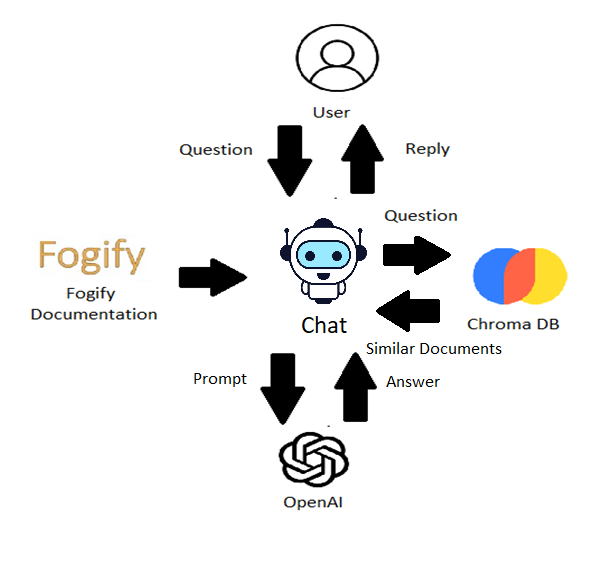
\includegraphics[width=8cm]{figures/methodology-pipline.png}
    \caption[Methodology pipline]{Methodology pipline for creating chatbot
        tool}
    \label{img:pipeline}
\end{figure}

To tackle our problem we create the methodology shown in image
\ref{img:pipeline}. Specifically, we use the documentation of the Fogify tool,
We started our process by creating the dataset form the Fogify documentation.
We focus on the html pages of the documentation. We filter out the different
metadata from the html webpages and keep only the useful data.

We use the OpenAI API to create embeddings for the data we extract and store it
in our vector database.
When we take a query from the user we perform prompt engineering to create a
sufficient
input for the LLM. In the promt engineering process we incorporate the Fogify
relevant results we get from the database. We use the prompt as input for the
LLM using the OpenAI API.

% More precisely we read all the documents with extension
% .xml, .html, .md, yaml. Then those documents are segmented into chunks of 1000
% characters. All those chunks form a list of document chunks.Then we need to
% transform this list into vectors. We achieve that by utilizing OpenAI in order
% to convert chunks to vector embeddings, those embeddings are stored in Chroma
% DB which is used for the persistent storage of the embeddings.After the above
% steps our tool is ready for use. More precisely, when the chat receives a user
% query, it searches the knowledge base in order to receive most relevant
% information (context) the we perform prompt engineering  ( context, user's
% question, memory of recent conversation messages between user and AI Model) and
% feed the prompy to AI model to get response